% !TEX TS-program = pdflatex
% !TEX encoding = UTF-8 Unicode
\documentclass[a4paper]{article}
\usepackage[swedish]{babel}
\usepackage[T1]{fontenc}
\usepackage[utf8]{inputenc}
\usepackage{mathtools}
\usepackage[pdftex]{graphicx}
\usepackage{float}
\usepackage{fancyhdr}
\usepackage{geometry}
\usepackage{booktabs} % for much better looking tables
\usepackage{array} % for better arrays (eg matrices) in maths
\usepackage{paralist} % very flexible & customisable lists (eg. enumerate/itemize, etc.)
\usepackage{verbatim} % adds environment for commenting out blocks of text & for better verbatim
\usepackage{subfig} % make it possible to include more than one captioned figure/table in a single float

%%% HEADERS & FOOTERS

\author{Jonathan Karlsson - jonka293 - 890201-1991 \and Niclas Olofsson - nicol271 - 900904-5338}
\pagestyle{fancy} % options: empty , plain , fancy
\renewcommand{\headrulewidth}{1pt} % customise the layout...
\fancyhead[LO,LE]{Laboration 1 - TDDC78}
\lfoot{}\cfoot{\thepage}\rfoot{}
\setlength{\parindent}{0pt}

%%%% SECTION TITLE APPEARANCE

%\usepackage{sectsty}
%\allsectionsfont{\sffamily\mdseries\upshape} % (See the fntguide.pdf for font help)
%% (This matches ConTeXt defaults)
%
%%%% ToC (table of contents) APPEARANCE
%\usepackage[nottoc,notlof,notlot]{tocbibind} % Put the bibliography in the ToC
%\usepackage[titles,subfigure]{tocloft} % Alter the style of the Table of Contents
%\renewcommand{\cftsecfont}{\rmfamily\mdseries\upshape}
%\renewcommand{\cftsecpagefont}{\rmfamily\mdseries\upshape} % No bold!

%%% END Article customizations

%%% The "real" document content comes below...

\title{Laboration 1 - TDDC78}

%\date{} % Activate to display a given date or no date (if empty),
% otherwise the current date is printed

\begin{document}

\maketitle

\section{Program description}
\subsection{Threshold filter}

This program calculates the average intensity of the image and makes all
pixels with a higher-than-average value white, and all other pixels
black.\\

The whole image is read on the root node. The root node also calculates
the  average intensity of the image. The calculated intensity is sent to
all other nodes via MPI\_Broadcast().\\

The image data array is split in as many parts as there are nodes, and
each node gets its own part via MPI\_Scatter(). Since each node needs to
know the data length to receive, this is done in two steps where the
total data length is first sent via MPI broadcast, and then the data is
sent with MPI scatter. Each node then runs the threshold filter on its
own part of the image. MPI\_Gather() then reassembles the resulting image,
which is written to disk by the root node.\\

\subsection{Blur filter}

For each pixel this program calculates the average color of the
neighbors with a given radius, of the pixel and sets the pixels color to
the average. This gives a blurred effect over the whole image with a
small radius giving almost the same image back, and a large radius gives a
very blurry image.\\

The whole image is read at the root node. The intervals that each
processor is going to work in is calculated. Since the algorithm is
dependent on the value of the neighbours of each pixels, we have to send
some more image information than we are actually blurring on each node,
otherwise there will be some broken lines in the image. The data is
distributed to the nodes using MPI\_Scatterv(). Now each chunk is
iterated by the blur filter and then transmitted to the root node with
MPI\_Gatherv(), the root node must take special care to get rid of some
overhead created by the sending of extra data. This is done by pointing
a bit forward in the array storing the image.

\section{Execution times}
In figure \ref{fig:fig1} and figure \ref{fig:fig4} the same number of nodes is used on different images and we see that the execution time is increased in a linear manor, for the thresh and blur filter. Figure \ref{fig:fig2} and figure \ref{fig:fig5} shows how the execution time decreases with increasing number of nodes for thresh and blur, in the thresh filter we get a bad scale since the problem size is so small that the communication overhead becomes too large. Figure \ref{fig:fig3} and figure \ref{fig:fig6} shows how the same increase in image size and number of nodes give the same execution time, for \ref{fig:fig6} we notice that the line isn\rq{}t constant as soon as we use more than one processor (more than 16 nodes).

\begin{figure}[h]
  \centering
  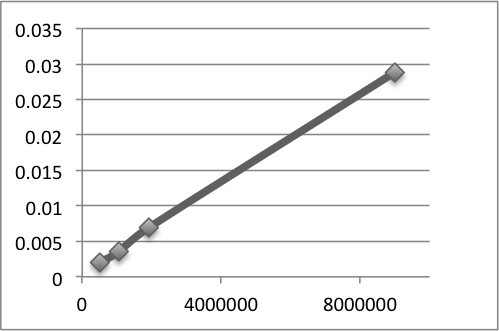
\includegraphics{sameProcessors.png}
  \caption{Using the same amount of nodes on different images. (Thresh)}
  \label{fig:fig1}
\end{figure}

\begin{figure}[h]
  \centering
  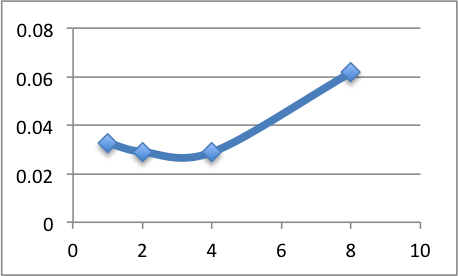
\includegraphics{samePixels.png}
  \caption{Using the same image with different number of nodes. (Thresh)}
  \label{fig:fig2}
\end{figure}

\begin{figure}[h]
  \centering
  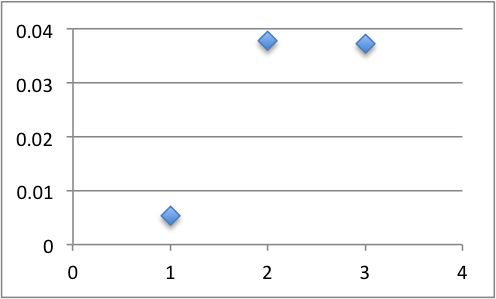
\includegraphics{samescale.png}
  \caption{Scaling the image at the same rate as the number of nodes. Using 2, 4 and 8 nodes. (Thresh)}
  \label{fig:fig3}
\end{figure}

\begin{figure}[h]
  \centering
  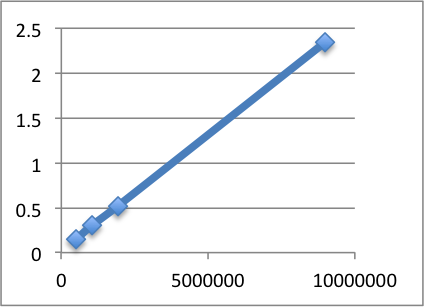
\includegraphics{sameProcessorBlur.png}
  \caption{Using the same amount of nodes on different images. (Blur)}
  \label{fig:fig4}
\end{figure}

\begin{figure}[h]
  \centering
  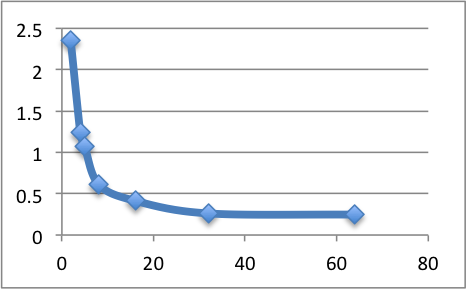
\includegraphics{samePixelsBlur.png}
  \caption{Using the same image with different number of nodes. (Blur)}
  \label{fig:fig5}
\end{figure}

\begin{figure}[h]
  \centering
  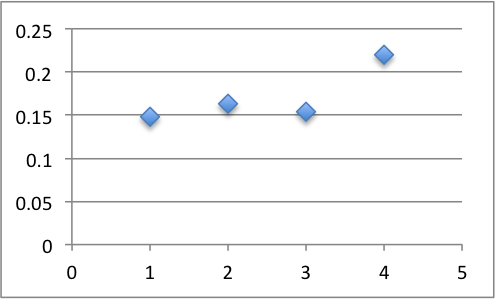
\includegraphics{sameDiffBlur.png}
  \caption{Scaling the image at the same rate as the number of nodes. Using 2, 4, 8 and 38 nodes. (Blur)}
  \label{fig:fig6}
\end{figure}

\end{document}
